% tools voor document
\documentclass{article} % definieer type document (article, resume, etc...)
\usepackage[english]{babel} % definieer taal van document

\usepackage[a4paper,top=2cm,bottom=2cm,left=3cm,right=3cm,marginparwidth=1.75cm]{geometry} % definieer formaat van document

% Handige packages
\usepackage{imakeidx} % package om indices te maken
\usepackage{amsmath} % package voor formules
\usepackage{graphicx} % package voor het invoegen van images
\usepackage{listings} % package voor het invoegen van listings (bron code)
\usepackage[colorlinks=true, allcolors=blue]{hyperref} % package voor hyperlinks (intern als extern)
\usepackage{xcolor} % package voor standaard kleuren
\usepackage{parskip} % package voor het formateren van paragraven
\usepackage{multirow} % package voor formateren tabellen --- \multicolumn{x}{|c|}{tekst}
\usepackage{ulem} % package om zinnen door te strepen met \sout{}
\usepackage[many]{tcolorbox} % for COLORED BOXES (tikz and xcolor included)

\usepackage{biblatex} %Imports biblatex package
\addbibresource{references.bib} %Import the bibliography file

% definieer kleuren: {naam}{kleurstijl}{waardes}
\definecolor{codegreen}{rgb}{0,0.6,0}
\definecolor{codegray}{rgb}{0.5,0.5,0.5}
\definecolor{codepurple}{rgb}{0.58,0,0.82}
\definecolor{backcolour}{rgb}{0.95,0.95,0.92}

% definieer stijl van lijsten
\lstdefinestyle{mystyle}{
    backgroundcolor=\color{backcolour},   
    commentstyle=\color{codegreen},
    keywordstyle=\color{magenta},
    numberstyle=\tiny\color{codegray},
    stringstyle=\color{codepurple},
    basicstyle=\ttfamily\footnotesize,
    breakatwhitespace=false,         
    breaklines=true,                 
    captionpos=b,                    
    keepspaces=true,                 
    numbers=left,                    
    numbersep=5pt,                  
    showspaces=false,                
    showstringspaces=false,
    showtabs=false,                  
    tabsize=2
}
\lstset{style=mystyle} % verander standaard stijl naar eigen stijl

\newtcolorbox{boxA}{
    fontupper = \bf,
    boxrule = 1.5pt,
    colframe = black % frame color
}

\hypersetup{
    colorlinks=true,
    linkcolor=blue,
    filecolor=magenta,      
    urlcolor=cyan,
    }
\urlstyle{same}

\begin{document}
%%%%%% TITLE PAGE %%%%%
\sffamily
\begin{titlepage}
    \centering
    \vfill
    {\bfseries\Huge
    Groepsverslag Tinlab Advanced Algorithms \\
    \vskip2cm
    }
    {\bfseries\Large
    Thijs Dregmans, Tobias de Bildt, Eliam Traas, Hidde-Jan Daniëls\\
    }
    {
    \bfseries\normalsize
    1024272, 1023603, 1003233, 0943798\\
    \vskip1cm
    \today\\
    }    
    \vfill
    
\includegraphics[width=4cm]{logohr.png} % also works with logo.pdf
    \vfill
    \vfill
\end{titlepage}
\newpage

%%%%% TABLE OF CONTENTS %%%%%
\tableofcontents
\newpage

%%%%% ANALYSE %%%%%
\section{Analyse}
Uit een analyse van het ministerie van Infrastructuur en Waterstaat (IenW) blijkt dat een groot aantal sluizen in Nederland de komende jaren aan renovatie toe zijn. De minister van Infrastructuur heeft opdracht gegeven voor het modelleren van sluizen om een beter beeld te krijgen van benodigde ontwerpkeuzes met betrekking tot - onder andere - veiligheid, efficiëntie, capaciteit, onderhoudskosten en duurzaamheid. Voordat requirements worden opgesteld, volgt een algemene analyse van het Nederlandse sluizenpark. \par

\subsection{Sluizen in Nederland}
Het Nederlandse sluizenpark bestaat uit een breed scala aan verschillende soorten sluizen. Het gaat niet alleen over sluizen voor de profesionele scheepvaart, maar bijvoorbeeld ook sluizen voor militaire doeleinden. Een voorbeeld hiervan is de \textit{'Plofsluis'} bij Nieuwegein. \cite{rijkswaterstaatPlofsluis} Sluizen met een militaire functie, zoals de Plofsluis, zijn vooral iets van het verleden. \par

Sluizen zijn in te delen in drie categorieën:
\begin{enumerate}
    \item Sluizen voor waterhuishouding
    \item Sluizen voor de scheepvaart
    \item Sluizen met een militaire functie
\end{enumerate}

\subsection{Soorten sluizen}
Vaak hebben sluizen meerdere functies. Het is dan bijvoorbeeld een grote sluis voor de scheepvaart, maar wordt ook gebruikt voor het watermanagement.\par

Onder de verschillende categorieën - die in feite functies van sluizen zijn - vallen een aantal typen. Voor de waterhuishouding bestaan er bijvoorbeeld zogenaamde ‘uitwateringssluizen’, ‘Ontlastsluizen’, ‘irrigatiesluizen’ en ‘keersluizen’. \par

De keersluis is een voorbeeld, waarbij de verschillende functies overlappen. Keersluizen worden vaak bij zeehavens aangelegd. Als het water te laag komt te staan, dan kan de keersluis worden gesloten om schade aan de haven en schepen door laag water worden voorkomen. De keersluis kan ook voor het omgekeerde gebruikt worden. Het heet dan een ‘doksluis’. In een dok worden schepen droog gebouwd. Met eb - als de dok droogstaat - wordt de sluis(deur) gesloten, zodat het water met hoogwater niet binnenkomt. Een keersluis heeft dus zowel een functie voor de waterhuishouding als voor de scheepvaart. \par

\subsection{Schutsluizen}
Het meest van de eerder genoemde sluizen kenmerkt zich door de enkele deuren. Hoewel het dus voorkomt dat een sluis voor de scheepvaart een enkele deur heeft - zoals de keersluis - zijn de meeste sluizen voor de scheepvaart schutsluizen. Schutsluizen kenmerken zich door de dubbele deuren. Ze verbinden twee waterwegen die een ongelijk waterpeil hebben. Door de deuren beurtelings te sluiten, water van de hoger gelegen waterweg naar binnen te pompen en de hoger gelegen deuren te openen, kunnen schepen eenvoudig over waterwegen getransporteerd worden, terwijl die waterwegen een ongelijk waterpeil hebben \cite{Arends1994}. \\
In de scheepvaart zijn de vrijwel alle sluizen, schutsluizen. Daarom ligt de focus in dit onderzoek op schutsluizen.
\newpage

\subsection{Werking van een schutsluis}
Een schutsluis heeft een aantal fases:
\begin{enumerate}
    \item Het schip vaart/de schepen varen de sluis binnen.
    \item De sluiskolk wordt gevuld of leeggepompt.
    \item Het schip vaart/de schepen varen de sluis uit.
\end{enumerate}
Bij een schutsluis zijn er minimaal 2 sluisdeuren. Ten alle tijde is er tenminste één deur gesloten. Anders zou het hebben van meerdere deuren zinloos zijn.

\subsubsection{Proces}
Er is sprake van een lager gelegen waterweg en een hoger gelegen waterweg. De lager gelegen waterweg noemen we \textbf{‘beneden’} en de hoger gelegen waterweg \textbf{‘boven’}.

\begin{boxA}
    \begin{itemize}
        \item In fase 1 is de bovenkant van de sluis gesloten. Beneden is geopend. Omdat de lagere deur geopend is, is het waterpeil in de sluis gelijk aan dat van het water stroomafwaarts.
        \item In fase 2 worden beide deuren gesloten. Het water in de sluis wordt op gelijke hoogte gebracht met dat stroomopwaarts.
        \item Als het water in de sluis op gelijke hoogte is als dat met het water stroomopwaarts, dan start fase 3. In fase 3 worden de sluisdeuren boven geopend en kan het schip de sluis uitvaren.
    \end{itemize}
\end{boxA}

Dit proces kan ook omgedraaid worden. In dat geval komt het schip de sluis van boven aanvaren. De sluisdeur boven gaat open wanneer het waterpeil gelijk is met dat van boven. Het schip vaart naar binnen. Het waterpeil in de sluis wordt gelijk gemaakt met dat van het water beneden. Vervolgens kunnen dan de sluisdeuren beneden open om het schip toegang tot de lager gelegen vaarweg te verlenen. \par

\subsubsection{Waterpeil bijstellen}
Water verplaatsen van boven naar beneden is niet moeilijk. Water stroomt van nature naar het laagste punt. Dit principe wordt in de sluizen gebruikt. Bij veel sluizen zijn er in de sluisdeuren luiken gemaakt, die tijdens fase 2 geopend kunnen worden. Door deze luiken te openen, kan er water vanuit de hoger of lager gelegen waterweg water naar of van de sluis worden gepompt. \par

\newpage
\subsubsection{Flowchart werking sluis}
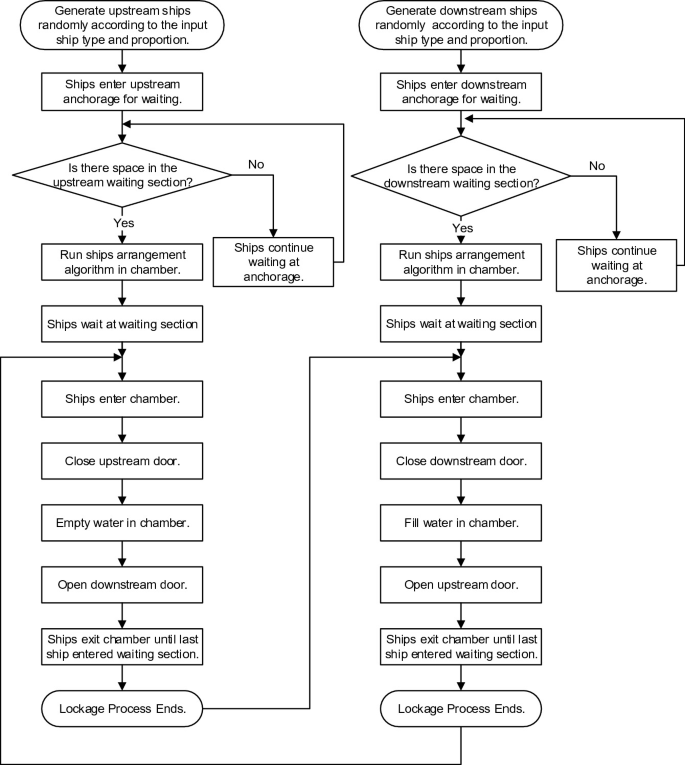
\includegraphics[width=0.9\textwidth]{lockageprocess.png} \cite{flowchart1}
\newpage

\subsection{Onderdelen van een schutsluis}
Een eenvoudige schutsluis bestaat uit enkele onderdelen:
\begin{enumerate}
    \item Sluisdeuren voor de afsluiting tussen sluis en waterweg stroomopwaarts.
    \item Sluisdeuren voor de afsluiting tussen sluis en waterweg stroomafwaarts.
    \item Luiken in de sluisdeuren stroomt opwaarts.
    \item Luiken in de sluisdeuren stroomafwaarts.
\end{enumerate}
De Grevelingensluis heeft een breedte van 16 meter en een lengte van 139 meter. Er mogen schepen in die minder dan 110 meter lang zijn. Dit wordt ook wel de \textbf{‘schutlengte’} genoemd. \cite{WaterkaartGrevelingensluis}

\subsection{Bediening van schutsluizen}
Bedieningstijden zijn veelal online te vinden. Rijkswaterstaat heeft een speciale website met reguliere openingstijden. Daarnaast is het vaak mogelijk om buiten deze tijden een afspraak te maken voor gebruik maken van een sluis. Als voorbeeld, in de sluisplanning van de volkeraksluizen valt af te lezen dat het ongeveer 20 á 30 minuten duurt. \cite{vaarweginformatie, volkeraksluizen, SluisplanningVolkeraksluizen} \par 

Wat betreft tijden, neemt fase 2 het grootste deel van de tijd in beslag. In een grote sluis zoals de Volkaraksluizen - waar jaarlijks zo’n 150.000 vrachtschepen passeren - worden in een paar minuten 900.000[note1] liters water verplaatst. \cite{WaterkaartVolkeraksluizen} Geschat wordt dat fase 2 zo’n 20 tot 25 minuten duurt, terwijl fase '1 en 3' 1 tot 3 minuten duren. \par

Na aanleiding van deze analyse definiëren wij de requirements, in lijn met de eisen gesteld door de opdrachtgever. \par


\begin{figure}[b]
    Note1: De sluis is 16 meter breedte en 139 meter lang. Er is een hoogte verschil van 0.40 meter. 0.4 * 16 * 139 = 889 kubieke meter.
\end{figure}
\newpage




%%%%% REQUIREMENTS
\section{Requirements}
De opdrachtgever heeft gesteld dat het doel is om tot een model van een volledig automatische sluis te komen. Hierbij wordt gehoopt op een verbetering in:
\begin{enumerate}
    \item Veiligheid
    \item Efficientie
    \item Capaciteit
    \item Duurzaamheid
\end{enumerate}

\subsection{Veiligheid}
We definiëren veiligheid als de afwezigheid van gevaar voor mens en bezit. De volgende situaties zijn gevaarlijk voor mens en/of bezit:
\begin{itemize}
    \item Beide deuren (boven en onder) zijn op hetzelfde moment geopend of zijn op hetzelfde moment in beweging. Dit zorgt - door het waterpeil verschil tussen boven en onder - voor een niet te stoppen stroom aan water. Dit kan voor gevaar zorgen.
    \item Een deur sluiten terwijl er een schip - of iets dergelijks - in de deuropening ligt.
    \item Een deur openen terwijl het waterpeil aan beide kanten van de deur ongelijk is. Dit zorgt voor een gevaarlijke stroom aan water - die vergelijkbaar is met punt 1.
    \item Er moeten seinen (stoplichten) aanwezig zijn voor de schepen die aangeven wanneer de schepen de sluis in of uit mogen varen.
\end{itemize}

\subsection{Efficientie}
Efficiëntie is de mate waarin de capaciteit maximaal benut wordt. Dit uit zich in:
\begin{itemize}
    \item De hoeveelheid schepen die de sluis per uur kan verwerken.
    \item Het aantal batches dat de sluis per uur kan verwerken.
\end{itemize}

Om de efficiëntie te maximaliseren wordt door de sluis gekeken naar de grootte van de rijen van wachtende schepen. De sluis geeft voorrang aan de rij schepen aan de kant van de sluis waar de deur geopend is. \\
Om de efficiëntie verder te verhogen, neemt de sluis de kleinst mogelijke hoeveelheid tijd om zowel de deuren te openen, te sluiten en de schepen naar binnen en naar buiten te laten varen.


\subsection{Capaciteit}
De capaciteit van een sluis kan worden opgevat op verschillende manieren:
\begin{itemize}
    \item De maximale grootte van een schip dat door de sluis kan varen.
    \item Het aantal schepen dat in een batch past.
\end{itemize}

Omdat de hoeveelheid schepen dat in een batch past, afhangt van de fysieke grootte van de sluis en de schepen, wordt de maximale grootte van de schepen buiten beschouwing gelaten. We maken deze keuze om een state-explosion te voorkomen.
Voor de modelleren nemen we aan dat alle schepen even groot zijn, en daarom is de maximale hoeveelheid schepen per batch constant. De capaciteit is het aantal schepen per batch. \par
Om de capaciteit te vergroten, probeert het model om de sluis zoveel als mogelijk schepen per batch te laten verwerken, tot de maximale capaciteit - aantal schepen per batch - is bereikt. \par
\newpage

\subsection{Duurzaamheid}
Duurzaamheid is ‘een ontwikkeling die voorziet in de behoeften van de huidige generatie, zonder de behoeften van toekomstige generaties, zowel hier als in andere delen van de wereld, in gevaar te brengen’. \cite{CBSduurzaamheid} \par

Dit heeft betrekking op de materiaalkeuze tijdens de bouw van de sluis. Omdat het model slechts een symbolische representatie van de sluis is, kan geen invloed worden uitgeoefend op de materialen. Daarom laten we de materiaalkeuze buiten beschouwing. \\
Een verbeterde duurzaamheid kan ook opgevat worden als het gebruik van een minimale hoeveelheid energie. Een sluis gebruikt energie voor verschillende zaken waarvan de belangrijkste de aansturing van de deuren en de pompen zijn. \\
Hoewel dit geen invloed heeft op het model, kunnen we energie besparen door pompen te vervangen door sluisluiken.

\subsection{Functionele requirements}
Bovengenoemde eisen zijn omgezet in de volgende functionele requirements:
\begin{enumerate}
    \item Er kan nooit een situatie ontstaan waarin niet ten minste één deur is gesloten.
    \item Een deur kan nooit gesloten worden, als er een schip in de deuropening ligt.
    \item Een deur kan nooit geopend worden, als het waterpeil aan beide kanten van de deur ongelijk is.
    \item Het invaarsein mag enkel en alleen op groen staan, als de bijbehorende deur geopend is en het uitvaarsein op rood staat.
    \item Het uitvaarsein mag enkel en alleen op groen staan, als de bijbehorende deur geopend is en het invaarsein op rood staat.
    \item Er kan op elk gegeven moment slechts één sein op groen staan.
    \item Als er schepen in de sluis liggen, heeft het uitvaarsein altijd voorrang op het invaarsein. Als alle schepen uit de sluis zijn gevaren, gaat het uitvaarsein uit en het invaarsein aan.
    \item Als er geen schip in de sluis ligt, dan gaat het uitvaarsein niet aan, maar het invaarsein gaat aan.
    \item De sluis wordt maximaal gevuld, tot óf het maximaal aantal schepen in de sluis is bereikt óf er geen wachtende schepen meer zijn die naar binnen kunnen varen.
    \item Als het maximaal aantal schepen in de sluis is bereikt of er zijn geen wachtende schepen meer, dan worden de deuren direct gesloten.
    \item Nadat de deuren zijn gesloten, duurt het maximaal 1 minuut totdat de sluisluiken geopend worden.
    \item Als het niveau aan beide kanten van de deuren gelijk is (na het openen van de luiken), duurt het maximaal 1 minuut tot de deuren geopend worden.
    \item Als er deuren geopend zijn, duurt het maximaal 1 minuut tot ofwel het invaar- of uitvaarsein aan gaat.
\end{enumerate}
\newpage

%%%%% MODELEREN %%%%%
\section{Modeleren}
\newpage

%%%%% VERIFICATIE %%%%%
\section{Verificatie}
\subsection{Testplan}
\subsection{Testrapport}
\subsection{Aanbevelingen}
\newpage


%%%%% BRONNEN %%%%%
\printbibliography
\end{document}
